\documentclass{standalone}
\usepackage{pgfplots}
\usetikzlibrary{shapes.geometric, intersections}
\pgfplotsset{compat=1.7}

\begin{document}
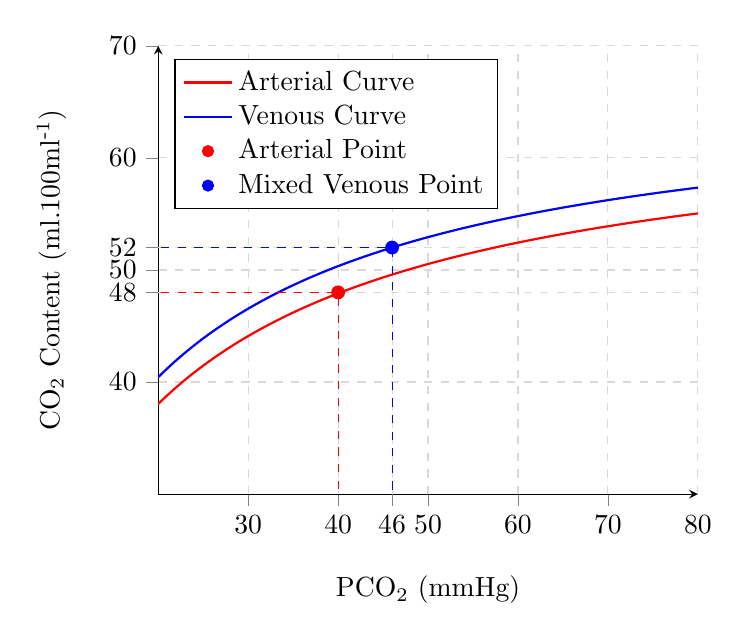
\begin{tikzpicture}

    \begin{axis}[
        axis lines=middle,
	ymin = 30,
	ymax = 70,
	xmin = 20,
xmax = 80,
        grid = major,
        grid style={dashed, gray!30},
	extra y ticks={48,52},
extra x ticks={46},
	 ylabel near ticks,
	xlabel near ticks,
        xlabel=PCO\textsubscript{2} (mmHg),
        ylabel=CO\textsubscript{2} Content (ml.100ml\textsuperscript{-1}),
        tick align=outside,
        enlargelimits=false,
legend entries={Arterial Curve,Venous Curve,Arterial Point,Mixed Venous Point},
    legend pos=north west,
legend cell align={left}]

	\addplot[domain=0:100, red, thick,samples=500] {(64.67682*x)/(13.99809 + x)};

	\addplot[domain=0:100, blue, thick,samples=500] {(66.99998*x)/(12.81369 + x) - 0.403};

	\draw[blue,thin,dashed] (axis cs: 0,52) -- (axis cs: 46, 52) node[circle,fill=blue,inner sep=0pt,minimum size=5pt]{} -- (axis cs: 46,0);
	\draw[red,thin,dashed] (axis cs: 0,48) -- (axis cs: 40,48) node[circle,fill=red,inner sep=0pt,minimum size=5pt]{} -- (axis cs: 40,0);

  \addlegendimage{only marks,red, mark=*}
    \addlegendimage{only marks,blue,mark=*}
    \addlegendimage{no markers,red}
    \addlegendimage{red}

\end{axis}

\end{tikzpicture} 
\end{document}